\subsection{Quality and time at $10^5$ points}
\label{sec:main}

\begin{table}[tbp]
\centering\scriptsize
\setlength{\tabcolsep}{3.2pt}
\caption{Mean excess over the certified optimum (\%) at $N=100{,}000$, square exact-fit
grid, instance seeds 1--3, one thread. The last two columns give the time of the certified
exact solver (seed 1) started from \ShuffleSnap-balanced (time included) or from
bisection. \textsuperscript{t}: no certificate within the 1-hour limit;
\textsuperscript{n}: stopped after 50 pricing rounds without a certificate. The bottom row
is the median time over all runs. Heavy tails are below 0.001\% for every method in
relative terms; Table~\ref{tab:abs} gives absolute excess.}
\label{tab:main}
\resizebox{\linewidth}{!}{\begin{tabular}{lrrrrrrrrrr}
\toprule
distribution & SS fast & BSP 16 & SS bal. & BSP 64 & SS qual. & RF master & RF PyPI & Bisect. & exact (s) & exact, bis. (s) \\
\midrule
uniform & 2.58 & 44.8 & 0.84 & 32.1 & 0.44 & 44.8 & 61.6 & 100.3 & 16.5 & 67.9 \\
Gaussian & $<$0.001 & 0.055 & $<$0.001 & 0.040 & $<$0.001 & 0.006 & 0.010 & 0.018 & 55.7 & 141 \\
Gaussian mixture & 0.013 & 5.61 & 0.002 & 3.74 & $<$0.001 & 16.7 & 16.7 & 12.3 & 94.6 & $>$3600\textsuperscript{t} \\
90/10 clusters & 0.050 & 0.032 & 0.012 & 0.019 & $<$0.001 & 1.16 & 1.16 & 0.57 & 214 & 1048 \\
ring & 0.005 & 1.16 & 0.001 & 0.95 & $<$0.001 & 41.0 & 41.0 & 40.3 & 114 & 3117 \\
spiral & 0.022 & 9.96 & 0.004 & 8.06 & 0.001 & 27.3 & 27.4 & 34.4 & 120 & 3331\textsuperscript{n} \\
checkerboard & 0.13 & 49.8 & 0.057 & 36.1 & 0.020 & 425.2 & 426.3 & 450.0 & 64.9 & 423 \\
heavy tails & $<$0.001 & $<$0.001 & $<$0.001 & $<$0.001 & $<$0.001 & $<$0.001 & $<$0.001 & $<$0.001 & 261 & 320 \\
duplicates & 0.15 & 12.3 & 0.038 & 5.44 & 0.013 & 49.0 & 49.0 & 39.3 & 1364 & $>$3600\textsuperscript{t} \\
near-line & 0.010 & 0.008 & 0.002 & 0.002 & $<$0.001 & 19.4 & 19.4 & 19.1 & 253 & $>$3600\textsuperscript{t} \\
\midrule
\emph{median time (s)} & 0.77 & 0.71 & 2.33 & 2.85 & 6.67 & 3.00 & 82.2 & 0.034 & 117 &  \\
\bottomrule
\end{tabular}
}
\end{table}

\begin{figure}[tbp]
  \centering
  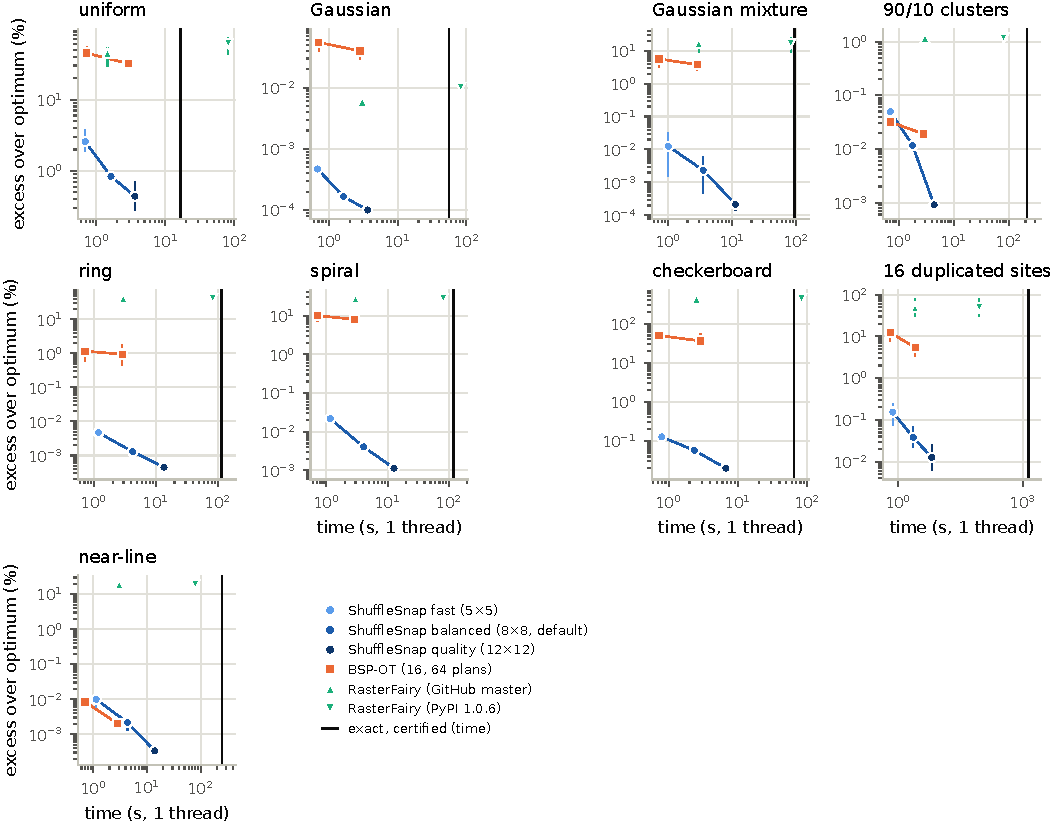
\includegraphics[width=\linewidth]{figures/fig_tradeoff_100k.pdf}
  \caption{Excess over the certified optimum against single-thread time at $N=100{,}000$
  (mean over three held-out instances; bars span min--max). The four \ShuffleSnap\ presets
  form the blue curve, from baseline to quality. BSP-OT at 16 and 64 plans is joined by an
  orange line. The black vertical line is the time of the certified exact solver.
  Heavy tails are omitted (all methods $<$0.001\%).}
  \label{fig:tradeoff}
\end{figure}

Table~\ref{tab:main} and Figure~\ref{fig:tradeoff} summarize the held-out comparison at
$10^5$ points on one thread.

\paragraph{\ShuffleSnap.} On nine of the eleven distributions, the baseline as specified
is within 0.2\% of the optimum, and on six of them within 0.03\%. It needs a median of
5\,s on one thread. The two exceptions are uniform points (2.5\%) and the jittered
lattice (33\%). There the optimum is small, so the long loops of
Section~\ref{sec:anatomy} dominate. The presets trade time for quality almost monotonically. The one exception is the
90/10 clusters, where fast is slightly worse than the baseline (0.034\% vs.\ 0.031\%). Balanced (median 16\,s) reduces the uniform excess to 0.84\%, and
quality (median 52\,s) to 0.44\%. The jittered lattice remains hard even for quality
(7.4\%): in absolute terms, 0.03 cells$^2$ per point against an optimum of 0.43
(Table~\ref{tab:abs}).

\paragraph{BSP-OT} is the fastest method (0.7\,s for 16 plans, 2.9\,s for 64). Its
excess, however, is typically 10--350$\times$ that of the \ShuffleSnap\ baseline:
32\% on uniform points, 36\% on the checkerboard, 8\% on the spiral and 3.7\% on the
mixture, all with 64 plans. It is competitive on two inputs. On the near-line, 64 plans
(0.002\%) match the balanced preset, and on the 90/10 clusters they beat the baseline
(0.019\% vs.\ 0.031\%) but not balanced (0.012\%).

\paragraph{RasterFairy (upstream)} takes about 3\,s. Its recursive slicing, however, costs
17--425\% on seven of the eleven distributions. It does well on three: the Gaussian
(0.006\%), the 90/10 clusters (1.2\%), and the jittered lattice, where it matches the
balanced preset (13.2\% vs.\ 12.7\%) because slicing a noisy lattice recovers the lattice.
The PyPI release, with pre-scaled inputs, gives similar or worse costs (e.g.\ 62\% vs.\ 45\%
on uniform points) and takes 80\,s at this size. Its targets at 50k and 100k points have a partially filled
last row, which sends it into its much slower mask code path; at $N=10^4$, a full
$100\times100$ square, it needs 0.03\,s.

\paragraph{With all cores.} On 24 hardware threads, \ShuffleSnap\ ran 13--15$\times$ faster than on
one and returned bit-identical assignments in all 396 paired runs. At $10^5$ points the
median time is 0.35\,s for the baseline, 1.1\,s for balanced and 3.9\,s for quality.
BSP-OT gained 4--7$\times$ (0.13\,s with 16 plans, 0.42\,s with 64); its plans are computed
in parallel, but the cycle-merging pass that combines them is largely sequential. At 24 threads, the baseline and BSP-OT with
64 plans therefore take about the same time, and the baseline has lower excess on nine of
the eleven distributions. The two exceptions are the near-line and the 90/10 clusters,
as above.

\paragraph{Exact solutions.} Started from \ShuffleSnap, the certified solver finished every
instance, in 7\,s (jittered lattice) to 23\,min (16 duplicated sites), with a median of
128\,s. That is 5--500$\times$ the time of the \ShuffleSnap\ baseline (median 25$\times$).
Started from bisection instead, it failed on four instances (mixture, duplicates,
near-line, spiral): no certificate within an hour or 50 pricing rounds. On six of the
seven instances where it did certify, it was 1.2--24$\times$ slower; on the jittered
lattice it was slightly faster (5\,s vs.\ 7\,s). The start matters because the candidate edges come from it:
\ShuffleSnap's layout is close enough to optimal that few pricing rounds are needed. A
dense exact solver is not an option at this size. Already at $N=10^4$, SciPy needed
3--352\,s (Table~\ref{tab:main10k} in the appendix), whereas the certified sparse solver
needed 0.3--7.7\,s.
